% =====================================================================
%  DEFENSA DE TESINA DE GRADO — LICENCIATURA EN CIENCIA DE DATOS
%  Universidad del Gran Rosario (UGR) — Rosario, Santa Fe, Argentina
%  Autores: Giuliano Crenna · Bruno Emmanuel Pace
%  Título: Detección temprana de indicios de depresión en publicaciones en español
%          mediante procesamiento del lenguaje natural
%  Subtítulo: Evaluación empírica de modelos contextuales y líneas base clásicas
%
%  Compatibilidad total:
%    - Tectonic: tectonic main.tex
%    - pdfLaTeX: pdflatex main.tex
%    - Overleaf: main.tex como documento principal (pdfLaTeX o XeLaTeX)
% =====================================================================

\documentclass[10pt,aspectratio=169]{beamer}

\usepackage{iftex}
\ifXeTeX
  \usepackage{fontspec}
\else\ifLuaTeX
  \usepackage{fontspec}
\else
  \usepackage[utf8]{inputenc}
  \usepackage[T1]{fontenc}
\fi\fi

\usepackage[spanish,es-tabla,es-nodecimaldot]{babel}
\usepackage{amsmath,amssymb}
\usepackage{graphicx}
\usepackage{xcolor}
\usepackage{booktabs}
\usepackage{colortbl}
\usepackage{tikz}
\usetikzlibrary{arrows.meta,fit,backgrounds,calc,shapes.geometric,decorations.pathreplacing,positioning}
\usepackage[most]{tcolorbox}
\usepackage{multicol}

% Rutas de recursos gráficos
\graphicspath{{figures/}{../figures/}{informe/figures/}{./}}

% ---------------------------------------------------------------------
% Paleta cromática institucional y académica (UGR)
% ---------------------------------------------------------------------
\definecolor{ugrAzul}{HTML}{0B3D91}
\definecolor{ugrCeleste}{HTML}{3FA9F5}
\definecolor{ugrRojo}{HTML}{E5323B}
\definecolor{ugrNaranja}{HTML}{E07B00}
\definecolor{ugrVerde}{HTML}{1E7E34}
\definecolor{ugrGris}{HTML}{555E68}
\definecolor{ugrFondoClaro}{HTML}{F4F8FC}
\definecolor{filaResaltada}{HTML}{E5F0FA}

% ---------------------------------------------------------------------
% Configuración estética de Beamer
% ---------------------------------------------------------------------
\usetheme{default}
\setbeamersize{text margin left=0.8cm,text margin right=0.8cm}
\usefonttheme{professionalfonts}
\setbeamertemplate{navigation symbols}{}

\setbeamercolor{structure}{fg=ugrAzul}
\setbeamercolor{title}{fg=ugrAzul}
\setbeamercolor{frametitle}{fg=ugrAzul}
\setbeamercolor{section in toc}{fg=ugrAzul}
\setbeamercolor{normal text}{fg=black}

% Encabezado compacto y elegante
\makeatletter
\setbeamertemplate{frametitle}{
  \vskip0.08cm
  \begin{beamercolorbox}[wd=\textwidth,sep=0pt,vmode]{frametitle}
    {\fontsize{12}{14}\selectfont\bfseries\color{ugrAzul}\insertframetitle}
    \ifx\insertframesubtitle\@empty\else
      \vskip1pt
      {\fontsize{8}{10}\selectfont\color{ugrGris}\textit{\insertframesubtitle}}
    \fi
  \end{beamercolorbox}
  \vskip1pt
  \textcolor{ugrCeleste!35}{\rule{\textwidth}{0.8pt}}
  \vskip0.10cm
}
\makeatother

% Pie de página discreto con logo UGR y contador
\setbeamertemplate{footline}{
  \leavevmode
  \hbox{%
    \begin{beamercolorbox}[wd=\paperwidth,ht=0.38cm,dp=0.12cm,leftskip=0.5cm,rightskip=0.5cm]{footline}%
      \raisebox{-0.04cm}{
\includegraphics[height=0.30cm]{logo_ugr.png}}%
      \hspace{0.25cm}%
      {\footnotesize\color{ugrGris}\insertsectionhead}%
      \hfill%
      {\footnotesize\bfseries\color{ugrAzul}%
        \insertframenumber\,/\,\inserttotalframenumber
      }%
    \end{beamercolorbox}%
  }%
  \vskip0.04cm
}

% Listas compactas
\setbeamertemplate{itemize item}{\textcolor{ugrAzul}{\scriptsize$\blacksquare$}}
\setbeamertemplate{itemize subitem}{\textcolor{ugrCeleste}{\scriptsize$\blacktriangleright$}}
\setbeamertemplate{itemize/enumerate body begin}{\setlength{\itemsep}{0.18em}\setlength{\parskip}{0pt}}
\setbeamerfont{itemize/enumerate body}{size=\small}
\setbeamerfont{itemize/enumerate subbody}{size=\footnotesize}

% ---------------------------------------------------------------------
% Cajas de contenido tcolorbox compactas
% ---------------------------------------------------------------------
\newcommand{\ugrblock}[2]{%
  \begin{tcolorbox}[
    enhanced, colback=ugrFondoClaro, colframe=ugrAzul, boxrule=0.7pt, arc=2.5pt,
    title={\textbf{#1}}, fonttitle=\footnotesize\bfseries, coltitle=white, colbacktitle=ugrAzul,
    left=6pt, right=6pt, top=4pt, bottom=4pt, before skip=0.15em, after skip=0.15em
  ]
    {\small #2}
  \end{tcolorbox}%
}

\newcommand{\ugrblockok}[2]{%
  \begin{tcolorbox}[
    enhanced, colback=ugrVerde!8, colframe=ugrVerde, boxrule=0.7pt, arc=2.5pt,
    title={\textbf{#1}}, fonttitle=\footnotesize\bfseries, coltitle=white, colbacktitle=ugrVerde,
    left=6pt, right=6pt, top=4pt, bottom=4pt, before skip=0.15em, after skip=0.15em
  ]
    {\small #2}
  \end{tcolorbox}%
}

\newcommand{\ugralert}[2]{%
  \begin{tcolorbox}[
    enhanced, colback=ugrNaranja!8, colframe=ugrNaranja, boxrule=0.7pt, arc=2.5pt,
    title={\textbf{#1}}, fonttitle=\footnotesize\bfseries, coltitle=white, colbacktitle=ugrNaranja,
    left=6pt, right=6pt, top=4pt, bottom=4pt, before skip=0.15em, after skip=0.15em
  ]
    {\small #2}
  \end{tcolorbox}%
}

% ---------------------------------------------------------------------
% Estilos TikZ para diagramas
% ---------------------------------------------------------------------
\tikzset{
    base/.style={rectangle, rounded corners=3pt, align=center, inner sep=3.5pt, line width=0.6pt},
    nodoES/.style={base, draw=ugrAzul, fill=ugrAzul!9, text width=3.1cm},
    nodoEN/.style={base, draw=ugrNaranja, fill=ugrNaranja!9, text width=3.1cm},
    proceso/.style={base, draw=ugrAzul, fill=white, text width=#1},
    resultado/.style={base, draw=ugrVerde, fill=ugrVerde!9, text width=#1},
    flecha/.style={-{Stealth[length=2.2mm, width=1.6mm]}, line width=0.7pt, color=ugrGris},
}

\newcommand{\tikzdiagram}[1]{%
  \begin{center}
    \resizebox{0.90\textwidth}{!}{#1}
  \end{center}%
}

% ---------------------------------------------------------------------
% Metadatos
% ---------------------------------------------------------------------
\title[Detección de depresión con PLN]{Detección temprana de indicios de depresión en publicaciones en español mediante procesamiento del lenguaje natural}
\subtitle{Evaluación empírica de modelos contextuales y líneas base clásicas}
\author[Crenna \& Pace]{Tec.\ Univ.\ Giuliano Crenna \and Tec.\ Univ.\ Bruno Emmanuel Pace}
\institute[UGR]{Universidad del Gran Rosario \\ Licenciatura en Ciencia de Datos}
\date{Rosario, 2026}

% =====================================================================
% CUERPO MODULAR
% =====================================================================
\begin{document}

% 1. Portada, Motivación y Planteamiento del Problema
% =====================================================================
% SECCIÓN 1: INTRODUCCIÓN, MOTIVACIÓN Y PROBLEMA
% =====================================================================

% ---------------------------------------------------------------------
% Diapositiva 1: Portada
% ---------------------------------------------------------------------
\begin{frame}[plain]
  \titlepage
  \note{
    Buenos días miembros del tribunal evaluador y docentes presentes. Hoy junto a Bruno Pace tenemos el agrado de presentar la defensa de nuestra tesina de grado para la Licenciatura en Ciencia de Datos de la Universidad del Gran Rosario, titulada: 'Detección temprana de indicios de depresión en publicaciones en español mediante procesamiento del lenguaje natural: Evaluación empírica de modelos contextuales y líneas base clásicas'.
  }
\end{frame}

% ---------------------------------------------------------------------
% Diapositiva 2: Contexto y Motivación
% ---------------------------------------------------------------------
\section{Comprensión del problema}

\begin{frame}{Contexto y motivación: salud pública y huella digital}
  
  \begin{columns}[T]
    \column{0.58\textwidth}
    \begin{itemize}
      \item \textbf{Crisis global de salud mental:} La depresión afecta a $\sim$5{,}2\,\% de los adultos del mundo (OMS, 2026) y es la principal causa de discapacidad persistente.
      \item \textbf{Brecha diagnóstica:} Hasta un 60\,\% de quienes padecen malestar afectivo no acceden a atención oportuna.
      \item \textbf{Huella digital en redes:} Señales lingüísticas y cambios conductuales en redes sociales meses antes de la primera consulta clínica.
      \item \textbf{Asimetría del español:} La investigación en PLN se concentra en \textbf{inglés}; en español los corpus anotados son escasos y de acceso restringido.
    \end{itemize}

    \column{0.40\textwidth}
    \begin{center}
      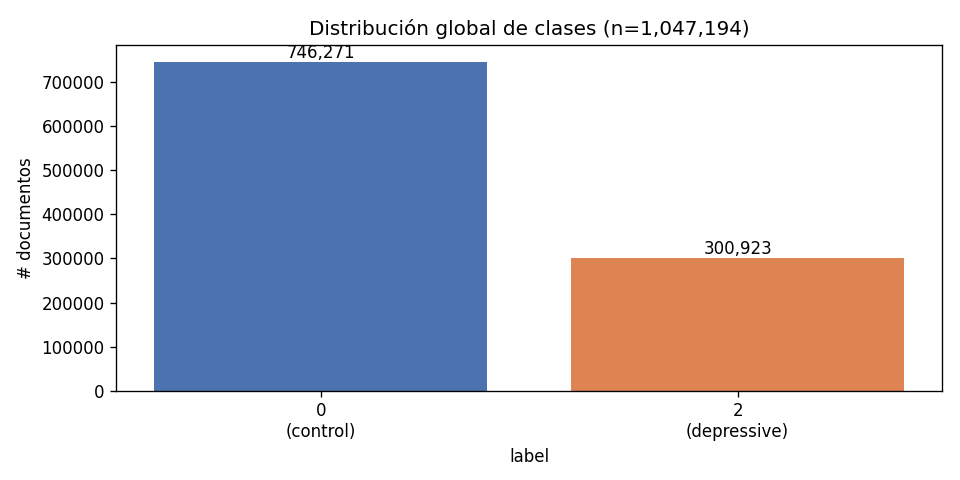
\includegraphics[width=\textwidth,height=0.34\textheight,keepaspectratio]{eda_02_distribucion_clases.png}
      \vskip-0.05cm
      {\tiny\color{ugrGris}Figura 1: Distribución global de clases en el corpus (1{,}31M de textos).\par}
    \end{center}
  \end{columns}

  \vskip0.05cm
  \ugrblock{Delimitación ética y alcance computacional}{
    Desarrollamos clasificadores estadísticos de texto como apoyo al cribado poblacional. El sistema \textbf{no} constituye ni sustituye un diagnóstico clínico.
  }

  \note{
    La depresión es una crisis de salud pública de escala mundial. Las redes sociales representan un canal donde los usuarios manifiestan cambios conductuales y léxicos tempranos. Sin embargo, existe una notable asimetría: casi toda la investigación en PLN se realiza en inglés, mientras que en español los recursos abiertos son mínimos. Aclaramos desde el inicio que el trabajo se enmarca en la clasificación supervisada para cribado preventivo, no en el diagnóstico médico.
  }
\end{frame}

% ---------------------------------------------------------------------
% Diapositiva 3: Planteamiento del Problema
% ---------------------------------------------------------------------
\begin{frame}{Planteamiento del problema y preguntas de investigación}
  \framesubtitle{Pregunta central y dimensiones metodológicas en Ciencia de Datos}

  \ugrblock{Pregunta central de investigación}{
    \textit{¿Es posible desarrollar un clasificador supervisado en Ciencia de Datos que, a partir de texto en español a nivel de publicación, distinga publicaciones con indicios de depresión frente a controles con un desempeño predictivo significativamente superior al de las representaciones clásicas, manteniendo robustez y evaluación no sesgada?}
  }

  \vskip0.05cm
  \begin{columns}[T]
    \column{0.49\textwidth}
    \ugrblock{1. Transferencia translingüística}{
      ¿Permite la traducción automática neuronal (EN$\to$ES) aumentar los datos de entrenamiento y beneficiar la detección en el dominio nativo en español?
    }
    \column{0.49\textwidth}
    \ugrblock{2. Evaluación por unidad de análisis}{
      ¿Cómo cambia el rendimiento predictivo al evaluar publicaciones individuales frente a perfiles completos de usuario?
    }
  \end{columns}

  \vskip0.05cm
  \begin{itemize}
    \item \textbf{Unidad de análisis:} Establecer una distinción metódica formal entre la predicción a \textbf{nivel de publicación} (tweet individual) y a \textbf{nivel de usuario} (perfil histórico acumulado).
  \end{itemize}

  \note{
    Formulamos una pregunta central con rigor epistemológico: contrastar si las arquitecturas Transformer contextuales superan efectivamente a los modelos clásicos en español bajo un marco no sesgado. A partir de allí exploramos si la traducción automática transfiere mejoras al dominio nativo.
  }
\end{frame}


% 2. Objetivos, Hipótesis y Metodología CRISP-DM
% =====================================================================
% SECCIÓN 2: MARCO METODOLÓGICO, OBJETIVOS E HIPÓTESIS
% =====================================================================

% ---------------------------------------------------------------------
% Diapositiva 4: Objetivos
% ---------------------------------------------------------------------
\begin{frame}{Objetivos de la investigación}
  \framesubtitle{Estructura articulada según la taxonomía de Bloom}

  \ugrblock{Objetivo general (Bloom 6 -- Crear)}{
    {\footnotesize Desarrollar un modelo de aprendizaje automático supervisado que, a partir de texto escrito en español, clasifique publicaciones de usuarios con indicios de sintomatología depresiva mediante un modelo de lenguaje contextual.}
  }

  \begin{columns}[T]
    \column{0.49\textwidth}
    \ugrblock{OE1 y OE2: Datos y líneas base}{
      {\scriptsize
      \begin{itemize}
        \item \textbf{OE1 -- Consolidar:} Integrar y estructurar un dataset masivo en español a partir de redes sociales.
        \item \textbf{OE2 -- Entrenar:} Entrenar clasificadores supervisados basados en representaciones léxicas TF-IDF.
      \end{itemize}}
    }
    \column{0.49\textwidth}
    \ugrblock{OE3 -- OE5: Contexto y evaluación}{
      {\scriptsize
      \begin{itemize}
        \item \textbf{OE3 -- Fine-tuning:} Ajuste fino supervisado de BETO.
        \item \textbf{OE4 -- Comparar:} Contraste empírico multidimensional.
        \item \textbf{OE5 -- Seleccionar:} Selección según significación ($p < 0{,}0005$), unidad de análisis y costo.
      \end{itemize}}
    }
  \end{columns}

  \note{
    Se definieron cinco objetivos específicos alineados con la taxonomía de Bloom: consolidar el corpus masivo integrado (OE1), entrenar líneas base léxicas (OE2), realizar el fine-tuning de BETO (OE3), comparar exhaustivamente los modelos (OE4) y seleccionar la arquitectura óptima según métricas y significación estadística (OE5).
  }
\end{frame}

% ---------------------------------------------------------------------
% Diapositiva 5: Hipótesis de Investigación y Protocolo Formal
% ---------------------------------------------------------------------
\begin{frame}{Hipótesis formal y protocolo de contraste}
  \framesubtitle{Criterio estadístico riguroso de decisión formal}

  \begin{columns}[T]
    \column{0.49\textwidth}
    \ugrblockok{Hipótesis de investigación ($H_1$)}{
      {\scriptsize Es posible desarrollar un modelo de aprendizaje automático supervisado que, a partir de texto escrito en español, clasifique publicaciones de usuarios con indicios de sintomatología depresiva mediante un modelo de lenguaje contextual.}
    }
    \column{0.49\textwidth}
    \ugrblock{Hipótesis nula ($H_0$)}{
      {\scriptsize No es posible desarrollar un modelo de aprendizaje automático supervisado que, a partir de texto escrito en español, clasifique publicaciones de usuarios con indicios de sintomatología depresiva mediante un modelo de lenguaje contextual.}
    }
  \end{columns}

  \vskip-0.05cm
  \ugrblock{Criterio de decisión formal (Bootstrap por conglomerados de usuarios)}{
    {\scriptsize Se define el contraste formal con $B = 2\,000$ réplicas remuestreando los 64 autores independientes del test nativo ($\alpha = 0{,}05$):
    \begin{equation*}
      \text{Rechazar } H_0 \text{ a favor de } H_1 \iff \Delta F_{1\text{-macro}}^{\text{low}} > 0 \;\land\; \Delta\text{AUC-ROC}^{\text{low}} > 0
    \end{equation*}
    donde $\Delta = \text{Métrica}(\text{BETO}_{\text{mono}}) - \text{Métrica}(\text{Mejor Línea Base})$. Los extremos inferiores del IC 95\,\% pareado deben excluir estrictamente el valor nulo ($0$).}
  }

  \note{
    La hipótesis se presenta verbatim conforme al informe final. La condición formal de rechazo de H0 exige que los extremos inferiores de los intervalos de confianza del 95\% para la diferencia pareada de F1-macro y AUC-ROC sean estrictamente positivos en el remuestreo de bootstrap por conglomerados de usuarios.
  }
\end{frame}

% ---------------------------------------------------------------------
% Diapositiva 6: Metodología CRISP-DM
% ---------------------------------------------------------------------
\begin{frame}{Metodología de trabajo: Enfoque CRISP-DM}
  \framesubtitle{Proceso estándar de minería de datos articulado en seis fases iterativas}

  \vskip-0.2cm
  \begin{center}
    \resizebox{0.88\textwidth}{!}{% Proceso de investigación según CRISP-DM (seis fases, recorrido en serpentina)
% Fila superior: 1 -> 2 -> 3. Fila inferior: 4 -> 5 -> 6 (de derecha a izquierda).
% Requiere los estilos proceso, resultado y flecha del documento anfitrión.
\begin{tikzpicture}[font=\footnotesize]
    \hyphenpenalty=10000\relax

    \tikzset{
        fase/.style={proceso=4.9cm, minimum height=3.0cm, align=left, anchor=center},
        iter/.style={-{Stealth[length=2.4mm, width=1.8mm]}, line width=0.8pt, color=ugrNaranja, dashed},
        ida/.style={{Stealth[length=2.4mm, width=1.8mm]}-{Stealth[length=2.4mm, width=1.8mm]}, line width=0.8pt, color=ugrGris},
    }

    \node[fase] (f1) at (-6.0, 0) {%
        {\small\bfseries\color{ugrAzul} 1. Comprensión del problema}\\[2pt]
        Pregunta, $H_1$/$H_0$ y objetivos\\
        Criterio de éxito: IC 95\,\% de $\Delta F_1$ y $\Delta$AUC $>0$\\
        Restricciones: tarea binaria, GPU de 8\,GB, corpus abiertos};

    \node[fase] (f2) at (0, 0) {%
        {\small\bfseries\color{ugrAzul} 2. Comprensión de los datos}\\[2pt]
        Cuatro fuentes: Twitter nativo y tres de Reddit traducido\\
        Análisis exploratorio, calidad y desbalance\\
        Distribución de clases y longitudes};

    \node[fase] (f3) at (6.0, 0) {%
        {\small\bfseries\color{ugrAzul} 3. Preparación de los datos}\\[2pt]
        Anonimización y traducción (MarianMT)\\
        Corpus unificado (1\,311\,023 textos)\\
        Partición 70/10/20 por usuario, rasgos y balanceo};

    \node[fase, draw=ugrAzul, fill=ugrAzul!8] (f4) at (6.0, -4.6) {%
        {\small\bfseries\color{ugrAzul} 4. Modelado}\\[2pt]
        TF-IDF con Regresión Logística y SVM\\
        Modelo combinado (19 rasgos)\\
        BETO; esquemas mono y multi};

    \node[fase, draw=ugrVerde, fill=ugrVerde!9] (f5) at (0, -4.6) {%
        {\small\bfseries\color{ugrAzul} 5. Evaluación}\\[2pt]
        $F_1$-macro, AUC, $\kappa$ y \emph{bootstrap} de 2\,000 réplicas\\
        Nivel de usuario y contraste formal\\
        Contraste de $H_0$};

    \node[fase] (f6) at (-6.0, -4.6) {%
        {\small\bfseries\color{ugrAzul} 6. Despliegue y cierre}\\[2pt]
        Código, manifiestos y predicciones reproducibles\\
        Uso no clínico y consideraciones éticas\\
        Informe y presentación};

    \draw[ida]   (f1) -- (f2);
    \draw[ida]   (f2) -- (f3);
    \draw[ida]   (f3) -- (f4);
    \draw[flecha] (f4) -- (f5);
    \draw[flecha] (f5) -- (f6);
    \draw[iter]  (f5.north west) -- node[midway, right=3pt, font=\scriptsize, text=ugrNaranja, align=left, inner sep=1pt] {nuevo\\ciclo} (f1.south east);

\end{tikzpicture}
}
  \end{center}
  \vskip-0.35cm
  {\scriptsize\centering\color{ugrGris}El flujo iterativo conecta la evaluación con la comprensión de datos y el modelado; el repositorio garantiza reproducibilidad con \texttt{make}.\par}

  \note{
    Adoptamos el estándar de Ciencia de Datos CRISP-DM en seis fases interconectadas. El ciclo conecta permanentemente la evaluación analítica con el preprocesamiento y el modelado. Todo el pipeline es reproducible mediante comandos en el Makefile del repositorio.
  }
\end{frame}


% 3. Corpus Masivo, Anonimización y Partición por Usuario
% =====================================================================
% SECCIÓN 3: COMPRENSIÓN Y PREPARACIÓN DE LOS DATOS
% =====================================================================

% ---------------------------------------------------------------------
% Diapositiva 7: Corpus Textual Masivo
% ---------------------------------------------------------------------
\section{Comprensión y preparación de datos}

\begin{frame}{Corpus textual masivo: fuentes y consolidación}
  \framesubtitle{1\,311\,023 publicaciones de 260\,357 usuarios en español}

  \begin{table}
    \centering\scriptsize
    \setlength{\tabcolsep}{5pt}
    \caption{Composición del corpus unificado (\texttt{corpus\_v1.parquet}).}
    \begin{tabular}{lrrll}
      \toprule
      \textbf{Fuente} & \textbf{Documentos} & \textbf{\%} & \textbf{Idioma orig.} & \textbf{Nivel de etiqueta} \\
      \midrule
      Coello-Guilarte (Twitter) & 1\,047\,194 & 79{,}88\,\% & Español (nativo) & Usuario completo (0 / 2) \\
      Kaggle SDD (Reddit) & 232\,067 & 17{,}70\,\% & Inglés (trad.) & Comunidad / autoinforme \\
      Reddit Mental Health Posts & 24\,031 & 1{,}83\,\% & Inglés (trad.) & Subreddit temático \\
      Depression Reddit & 7\,731 & 0{,}59\,\% & Inglés (trad.) & Subreddit temático \\
      \midrule
      \textbf{Total consolidado} & \textbf{1\,311\,023} & \textbf{100\,\%} & -- & \textbf{260\,357 usuarios} \\
      \bottomrule
    \end{tabular}
  \end{table}

  \vskip-0.15cm
  \begin{columns}[T]
    \column{0.49\textwidth}
    \ugrblock{Anonimización y privacidad}{
      \begin{itemize}
        \item Supresión de URLs, menciones (@usuario), correos y teléfonos.
        \item Identificadores hasheados con SHA-256 (prefijo de 12 hex).
      \end{itemize}
    }
    \column{0.49\textwidth}
    \ugrblock{Calidad y multimodalidad}{
      \begin{itemize}
        \item Textos vacíos residuales inferiores al 0{,}02\,\%.
        \item Registro dual: microtexto de Twitter (14 tokens) vs.\ publicaciones extensas de Reddit (112 tokens).
      \end{itemize}
    }
  \end{columns}

  \note{
    Consolidamos un corpus inédito de más de 1,3 millones de textos anonimizados. La fuente nativa en español reúne 317 usuarios clínicos de Twitter, a los que sumamos tres colecciones de Reddit traducidas con redes neuronales para evaluar la transferencia de dominio. Toda la información personal fue eliminada de forma irreversible.
  }
\end{frame}

% ---------------------------------------------------------------------
% Diapositiva 8: Partición a Nivel de Usuario
% ---------------------------------------------------------------------
\begin{frame}{Partición estricta a nivel de usuario (prevención de fuga)}
  \framesubtitle{Estratificación 70/10/20 agrupada por autor (semilla fija 42)}

  \vskip-0.1cm
  \tikzdiagram{% Partición independiente por fuente: cada corpus se divide 70/10/20 por usuario.
\begin{tikzpicture}[font=\footnotesize, x=1cm, y=1cm]
    % Leyenda
    \node[anchor=west] at (0, 1.3) {%
        \tikz\fill[ugrAzul] (0,0) rectangle (0.3,0.3); Entrenamiento (70\,\%)\qquad
        \tikz\fill[ugrCeleste] (0,0) rectangle (0.3,0.3); Validación (10\,\%)\qquad
        \tikz\fill[ugrNaranja] (0,0) rectangle (0.3,0.3); Prueba (20\,\%)};

    % Barras por fuente
    \foreach \y/\nombre/\info in {
        0/Coello-Guilarte/317 usuarios,
        -1.05/Kaggle SDD/232\,067 usuarios sintéticos,
        -2.1/Reddit MH Posts/20\,242 usuarios,
        -3.15/Depression Reddit/7\,731 usuarios sintéticos} {
        \node[anchor=east, align=right] at (-0.25, \y) {\textbf{\nombre}\\[-1pt] {\color{ugrGris}\info}};
        \fill[ugrAzul]    (0, \y - 0.32) rectangle (7, \y + 0.32);
        \fill[ugrCeleste] (7, \y - 0.32) rectangle (8, \y + 0.32);
        \fill[ugrNaranja] (8, \y - 0.32) rectangle (10, \y + 0.32);
        \draw[white, line width=1.4pt] (7, \y - 0.32) -- (7, \y + 0.32) (8, \y - 0.32) -- (8, \y + 0.32);
        \node[text=white, font=\scriptsize\bfseries] at (3.5, \y) {usuarios completos, estratificados por clase};
    }

    % Test nativo común
    \draw[ugrRojo, line width=1.1pt, dashed, rounded corners=2pt] (7.92, -0.42) rectangle (10.08, 0.42);
    \node[ugrRojo, anchor=south, font=\scriptsize\bfseries] at (9.0, 0.44) {test nativo común};

    % Llaves
    \draw[decorate, decoration={brace, amplitude=5pt}, line width=0.8pt, ugrAzul] (10.35, 0.36) -- (10.35, -0.36)
        node[midway, right=7pt, text=ugrAzul] {\textbf{splits mono}};
    \draw[decorate, decoration={brace, amplitude=7pt}, line width=0.8pt, ugrNaranja!90!black] (12.75, 0.42) -- (12.75, -3.5)
        node[midway, right=9pt, align=left, text=ugrNaranja!90!black] {\textbf{splits multi}\\ unión de las\\ cuatro fuentes};
\end{tikzpicture}
}

  \vskip-0.15cm
  \begin{columns}[T]
    \column{0.49\textwidth}
    \ugralert{El riesgo de fuga (\emph{Data Leakage})}{
      Si se divide al azar por documento, textos del mismo autor caen en entrenamiento y prueba: el clasificador aprende a reconocer al autor en vez de la señal afectiva.
    }
    \column{0.49\textwidth}
    \ugrblockok{Blindaje metodológico}{
      Todos los textos de un usuario permanecen en un único conjunto. El \textbf{test nativo común} cuenta con \textbf{64 usuarios nunca vistos} en entrenamiento (250\,847 tweets reales).
    }
  \end{columns}

  \note{
    Uno de los pilares del trabajo es evitar el data leakage: agrupar la partición por autor. De esta forma, los 64 autores del conjunto de prueba nativo son completamente desconocidos para los modelos, garantizando una evaluación predictiva genuina sobre nuevos sujetos.
  }
\end{frame}

% ---------------------------------------------------------------------
% Diapositiva 9: Pipeline de Traducción y Preprocesamiento
% ---------------------------------------------------------------------
\begin{frame}{Pipeline de traducción y extracción de rasgos}
  \framesubtitle{Traducción neuronal y enriquecimiento psicolingüístico}

  \begin{columns}[T]
    \column{0.49\textwidth}
    \ugrblock{Traducción automática neuronal}{
      \begin{itemize}
        \item Modelo Transformer \textbf{MarianMT} (\texttt{opus-mt-en-es}).
        \item 263\,829 publicaciones traducidas con caché JSONL.
        \item Control de consistencia sintáctica y semántica.
      \end{itemize}
    }
    \vskip0.05cm
    \ugrblock{Balanceo de clases (solo entrenamiento)}{
      \begin{itemize}
        \item \textbf{Submuestreo 50/50:} 424\,436 textos en mono (usado en BETO para eficiencia en GPU).
        \item \textbf{Ponderación de clases:} 700\,717 textos en mono ($w_c \propto 1 / n_c$).
      \end{itemize}
    }

    \column{0.49\textwidth}
    \ugrblock{19 Rasgos psicolingüísticos y temporales}{
      Inspirados en la literatura psiquiátrica (LIWC) adaptados al español:
      \begin{itemize}
        \item \textbf{Foco en sí mismo:} Pronombres y verbos en 1ª persona del singular (\emph{yo, me, mi, conmigo}).
        \item \textbf{Pensamiento absolutista:} Términos cognitivos rígidos (\emph{siempre, nunca, jamás, nada, todo}).
        \item \textbf{Léxico afectivo:} Emociones NRC en español y polaridad léxica VADER.
        \item \textbf{Patrones temporales:} Hora de publicación y signos de insomnio o vigilia nocturna.
      \end{itemize}
    }
  \end{columns}

  \note{
    Para traducir Reddit utilizamos MarianMT en un pipeline local con caché para asegurar reproducibilidad. Paralelamente, implementamos un módulo para extraer 19 rasgos psicolingüísticos clásicos basados en Pennebaker: autorreferencia excesiva, absolutismo y polaridad afectiva, excluyendo cualquier rasgo derivado de la cantidad de mensajes para evitar fuga.
  }
\end{frame}


% 4. Jerarquía de Modelos y Arquitectura BETO
% =====================================================================
% SECCIÓN 4: MODELADO Y ARQUITECTURA
% =====================================================================

% ---------------------------------------------------------------------
% Diapositiva 10: Jerarquía de Modelos Supervisados
% ---------------------------------------------------------------------
\section{Modelado}

\begin{frame}{Jerarquía de modelos supervisados}
  \framesubtitle{Tres niveles de complejidad representacional y diseño experimental $2 \times 2$}

  \begin{columns}[T]
    \column{0.32\textwidth}
    \ugrblock{1. Líneas base léxicas}{
      {\scriptsize
      \begin{itemize}
        \item \textbf{TF-IDF:} Unigramas y bigramas ($V = 15\,000$).
        \item \textbf{Regresión Logística:} Regularización $L_2$ ($C=1{,}0$).
        \item \textbf{SVM lineal:} Margen con norma $L_2$.
      \end{itemize}}
    }

    \column{0.33\textwidth}
    \ugrblock{2. Modelo combinado}{
      {\scriptsize
      \begin{itemize}
        \item \textbf{Enriquecimiento:} TF-IDF + 19 rasgos psicolingüísticos.
        \item \textbf{Clasificador:} LR calibrada.
        \item \textbf{Objetivo:} Evaluar si rasgos expertos superan n-gramas.
      \end{itemize}}
    }

    \column{0.33\textwidth}
    \ugrblockok{3. Modelo contextual}{
      {\scriptsize
      \begin{itemize}
        \item \textbf{BETO:} Transformer preentrenado (\texttt{dccuchile}).
        \item \textbf{Capacidad:} 110M params (\emph{fine-tuning}).
        \item \textbf{Atención:} Orden, polisemia y negaciones sintácticas.
      \end{itemize}}
    }
  \end{columns}

  \vskip-0.10cm
  \ugrblock{Diseño experimental $2 \times 2$ (Mono vs.\ Multi)}{
    {\scriptsize Cada familia se entrenó en dos modalidades: \textbf{Mono} (solo Twitter nativo) y \textbf{Multi} (Twitter + Reddit traducido), evaluadas sobre el conjunto nativo de prueba común.}
  }

  \note{
    Planteamos una progresión metodológica rigurosa: líneas base léxicas puras (TF-IDF con Regresión Logística y SVM); un modelo combinado que incorpora los 19 rasgos psicolingüísticos; y el modelo contextual de vanguardia BETO. Cada modelo se entrena en modalidad mono y multi para comparar el impacto del aumento de datos.
  }
\end{frame}

% ---------------------------------------------------------------------
% Diapositiva 11: Arquitectura de BETO y Configuración Experimental
% ---------------------------------------------------------------------
\begin{frame}{Arquitectura de BETO y configuración experimental}
  \framesubtitle{Ajuste fino supervisado con restricciones computacionales reales}

  \begin{columns}[T]
    \column{0.48\textwidth}
    \begin{center}
      \resizebox{0.88\columnwidth}{!}{% Arquitectura del ajuste fino de BETO para clasificación binaria.
\begin{tikzpicture}[font=\footnotesize, node distance=0.55cm]
    \node[proceso=2.6cm, fill=ugrGris!8, draw=ugrGris] (tx) {\textbf{Texto}\\ \emph{``no me}\\ \emph{siento bien''}};
    \node[proceso=2.6cm, right=of tx] (tok) {\textbf{Tokenización}\\ WordPiece\\ \texttt{[CLS]} \dots{} \texttt{[SEP]}\\ máx.\ 128 tokens};
    \node[proceso=2.9cm, right=of tok, minimum height=2.6cm, fill=ugrAzul!10, line width=0.9pt] (enc)
        {\textbf{BETO}\\ codificador Transformer\\ 12 capas \texttimes{} 12 cabezas\\ $d = 768$\\ {\color{ugrGris}\scriptsize preentrenado, se ajusta}};
    \node[proceso=2.2cm, right=of enc] (cls) {\textbf{Vector}\\ $h_{\texttt{[CLS]}} \in \mathbb{R}^{768}$};
    \node[proceso=2.2cm, right=of cls, draw=ugrNaranja, fill=ugrNaranja!8] (lin) {\textbf{Capa lineal}\\ $768 \to 2$\\ + softmax};
    \node[resultado=2.9cm, below=0.7cm of lin] (out) {$P(\text{depresivo}\mid x)$};

    \draw[flecha] (tx) -- (tok);
    \draw[flecha] (tok) -- (enc);
    \draw[flecha] (enc) -- (cls);
    \draw[flecha] (cls) -- (lin);
    \draw[flecha] (lin) -- (out);
    \node[below=0.15cm of enc, font=\scriptsize, text=ugrGris, align=center] {AdamW, $\eta = 2\times10^{-5}$, lote 16, FP16};
\end{tikzpicture}
}
      \vskip0.05cm
      {\tiny\color{ugrGris}Diagrama: WordPiece $\to$ BETO ($d=768$) $\to$ Capa lineal $\to$ Softmax.\par}
    \end{center}

    \column{0.50\textwidth}
    \ugrblock{Configuración de hiperparámetros y hardware}{
      {\scriptsize
      \begin{itemize}
        \item \textbf{Optimizador:} AdamW ($\text{weight decay} = 0{,}01$, $\eta = 2 \times 10^{-5}$).
        \item \textbf{Secuencia y lote:} Longitud máx.\ 128 tokens, lote de 16.
        \item \textbf{Entrenamiento:} 3 épocas con \emph{early stopping} (óptimo en época 2).
        \item \textbf{Hardware:} GPU NVIDIA RTX 3060 Ti (8\,GB VRAM) en FP16.
      \end{itemize}}
    }
  \end{columns}

  \note{
    BETO procesa la secuencia tokenizada con WordPiece; el vector contextual de la salida CLS en la capa 12 alimenta una capa lineal hacia dos neuronas con softmax. El ajuste fino se completó en hardware local mediante precisión mixta FP16, alcanzando el óptimo en la época 2.
  }
\end{frame}

% ---------------------------------------------------------------------
% Diapositiva 12: Ejemplo de Clasificación End-to-End
% ---------------------------------------------------------------------
\begin{frame}{Ejemplo de Clasificación End-to-End}
  \framesubtitle{Flujo secuencial de inferencia sobre una publicación individual}

  \vskip-0.1cm
  \begin{center}
  \resizebox{0.96\textwidth}{!}{
  \begin{tikzpicture}[
    paso/.style={rectangle, rounded corners=4pt, draw=ugrAzul, fill=ugrFondoClaro, line width=0.8pt, inner sep=6pt, align=center, text width=3.0cm, font=\small},
    pasoOk/.style={rectangle, rounded corners=4pt, draw=ugrVerde, fill=ugrVerde!10, line width=0.8pt, inner sep=6pt, align=center, text width=3.0cm, font=\small},
    flechaFlujo/.style={-{Stealth[length=2.5mm, width=1.8mm]}, line width=1.2pt, color=ugrCeleste}
  ]
    % Nodos
    \node[paso] (n1) at (0, 0) {
      \textbf{\color{ugrAzul}1. Texto de entrada}\\[3pt]
      {\scriptsize Publicación individual}\\[4pt]
      \emph{\tiny ``Nunca me sentí tan vacío, no le encuentro sentido a nada...''}
    };

    \node[paso] (n2) at (3.8, 0) {
      \textbf{\color{ugrAzul}2. Tokenización}\\[3pt]
      {\scriptsize WordPiece ($V = 31\text{k}$)}\\[4pt]
      \texttt{\tiny [CLS] nunca me sentí tan vacío , no le encuentro ... [SEP]}\\[3pt]
      {\tiny Longitud $L = 128$}
    };

    \node[paso] (n3) at (7.6, 0) {
      \textbf{\color{ugrAzul}3. Modelo BETO}\\[3pt]
      {\scriptsize Transformer Bidireccional}\\[4pt]
      {\tiny 12 capas $\cdot$ 110M params}\\[2pt]
      {\tiny Vector contextual}\\[2pt]
      \textbf{\tiny $\mathbf{h}_{\text{[CLS]}} \in \mathbb{R}^{768}$}
    };

    \node[pasoOk] (n4) at (11.4, 0) {
      \textbf{\color{ugrVerde}4. Predicción}\\[3pt]
      {\scriptsize Capa lineal + Softmax}\\[4pt]
      {\tiny $P(\text{Depresión}) = \mathbf{0{,}89}$}\\[2pt]
      {\tiny $P(\text{Control}) = 0{,}11$}\\[3pt]
      \textbf{\footnotesize\color{ugrRojo}Indicios de depresión}
    };

    % Flechas
    \draw[flechaFlujo] (n1) -- (n2);
    \draw[flechaFlujo] (n2) -- (n3);
    \draw[flechaFlujo] (n3) -- (n4);
  \end{tikzpicture}
  }
  \end{center}

  \vskip0.05cm
  \begin{columns}[T]
    \column{0.49\textwidth}
    \ugrblock{Captura contextual vs.\ bolsa de palabras}{
      BETO preserva el orden secuencial y resuelve la negación (\emph{``no le encuentro sentido''}), que los modelos léxicos dispersan en términos inconexos.
    }
    \column{0.49\textwidth}
    \ugrblockok{Salida probabilística calibrada}{
      La distribución de salida provee una probabilidad posterior interpretable, permitiendo ajustar umbrales de decisión según la sensibilidad clínica requerida.
    }
  \end{columns}

  \note{
    Ilustramos el pipeline de clasificación end-to-end: desde el microtexto crudo hasta la probabilidad final. El texto pasa por la tokenización WordPiece con tokens especiales CLS y SEP; las 12 capas de auto-atención de BETO generan el embedding contextual de 768 dimensiones, y la capa lineal clasifica la publicación con una probabilidad de indicios de depresión del 89\%.
  }
\end{frame}


% 5. Protocolo de Evaluación, Resultados y Contrastación Formal
% =====================================================================
% SECCIÓN 5: RESULTADOS PRINCIPALES Y CONTRASTACIÓN FORMAL
% =====================================================================

% ---------------------------------------------------------------------
% Diapositiva 12: Protocolo y Métricas
% ---------------------------------------------------------------------
\section{Evaluación}

\begin{frame}{Protocolo de evaluación y métricas multidimensionales}
  \framesubtitle{Evaluación robusta ante desbalance y estimación de incertidumbre}

  \begin{columns}[T]
    \column{0.52\textwidth}
    \begin{itemize}
      \item \textbf{Métrica rectora ($F_1$-macro):} Media armónica no ponderada entre ambas clases; balancea control y depresión.
      \item \textbf{Sensibilidad clínica ($F_1$-depresión):} Rendimiento exclusivo sobre la clase positiva de interés.
      \item \textbf{Discriminación (AUC-ROC):} Capacidad probabilística independiente del umbral de corte.
      \item \textbf{Acuerdo por azar ($\kappa$ de Cohen):} Fiabilidad ajustada por la prevalencia de las clases.
    \end{itemize}

    \column{0.46\textwidth}
    \ugrblock{Incertidumbre por Bootstrap ($B=2\,000$)}{
      \begin{itemize}
        \item \textbf{Conglomerados por usuario:} Remuestreo en bloque de los 64 autores del test nativo común.
        \item \textbf{Independencia real:} Conserva intacta la estructura correlacionada de textos por autor.
        \item \textbf{Intervalos de confianza:} Método percentil empírico del 95\,\% ($[\alpha/2;\; 1 - \alpha/2]$).
      \end{itemize}
    }
  \end{columns}

  \note{
    Ante el desbalance de clases, seleccionamos F1-macro como métrica principal y AUC-ROC como métrica umbral-independiente. Para medir la variabilidad real, aplicamos un bootstrap de conglomerados de 2000 réplicas sobre los 64 usuarios del conjunto de prueba, respetando la correlación intra-sujeto.
  }
\end{frame}

% ---------------------------------------------------------------------
% Diapositiva 13: Resultados en el Test Nativo Común
% ---------------------------------------------------------------------
\begin{frame}{Resultados principales sobre el test nativo común}
  \framesubtitle{Evaluación sobre 250\,847 tweets de 64 usuarios independientes}

  \begin{table}
    \centering\scriptsize
    \setlength{\tabcolsep}{4pt}
    \caption{Métricas con intervalos de confianza del 95\,\% (Bootstrap de 64 usuarios, $B=2\,000$).}
    \begin{tabular}{lcccc}
      \toprule
      \textbf{Modelo evaluado} & \textbf{F1-macro} & \textbf{F1 depresión} & \textbf{AUC-ROC} & \textbf{Kappa ($\boldsymbol{\kappa}$)} \\
      \midrule
      LR TF-IDF (submuestreo) & 0{,}653 \tiny{[0{,}605; 0{,}691]} & 0{,}544 & 0{,}753 \tiny{[0{,}715; 0{,}788]} & 0{,}317 \\
      LR TF-IDF (ponderado) & 0{,}655 \tiny{[0{,}606; 0{,}693]} & 0{,}546 & 0{,}755 \tiny{[0{,}718; 0{,}790]} & 0{,}321 \\
      SVM lineal TF-IDF & 0{,}653 \tiny{[0{,}605; 0{,}692]} & 0{,}544 & 0{,}754 \tiny{[0{,}716; 0{,}787]} & 0{,}318 \\
      LR Combinado (19 rasgos) & 0{,}644 \tiny{[0{,}593; 0{,}684]} & 0{,}540 & 0{,}750 \tiny{[0{,}710; 0{,}785]} & 0{,}303 \\
      \rowcolor{filaResaltada}
      \textbf{BETO mono (contextual)} & \textbf{0{,}717} \tiny{[0{,}665; 0{,}759]} & \textbf{0{,}613} & \textbf{0{,}808} \tiny{[0{,}755; 0{,}849]} & \textbf{0{,}437} \\
      \bottomrule
    \end{tabular}
  \end{table}

  \vskip-0.15cm
  \begin{columns}[T]
    \column{0.49\textwidth}
    \ugrblockok{Superioridad de BETO}{
      BETO supera a la mejor línea base léxica en \textbf{+6{,}2 puntos de F1-macro} y \textbf{+5{,}2 puntos de AUC-ROC}.
    }
    \column{0.49\textwidth}
    \ugralert{Hallazgo sobre rasgos expertos}{
      Los 19 rasgos psicolingüísticos \textbf{no superaron} a los n-gramas puros (F1 0{,}644 vs.\ 0{,}655); el vocabulario absorbe la señal.
    }
  \end{columns}

  \note{
    En el conjunto nativo común, las líneas base clásicas convergen en 0.655 de F1-macro y 0.755 de AUC. Los rasgos psicolingüísticos no aportan ganancia frente al TF-IDF. Por su parte, BETO mono alcanza 0.717 de F1-macro y 0.808 de AUC, logrando una diferencia sustantiva superior a 6 puntos porcentuales.
  }
\end{frame}

% ---------------------------------------------------------------------
% Diapositiva 14: Discriminación y Curvas ROC
% ---------------------------------------------------------------------
\begin{frame}{Capacidad de discriminación y matriz de confusión}
  \framesubtitle{Análisis de curvas ROC y estructura de clasificación de BETO}

  \begin{columns}[T]
    \column{0.50\textwidth}
    \begin{center}
      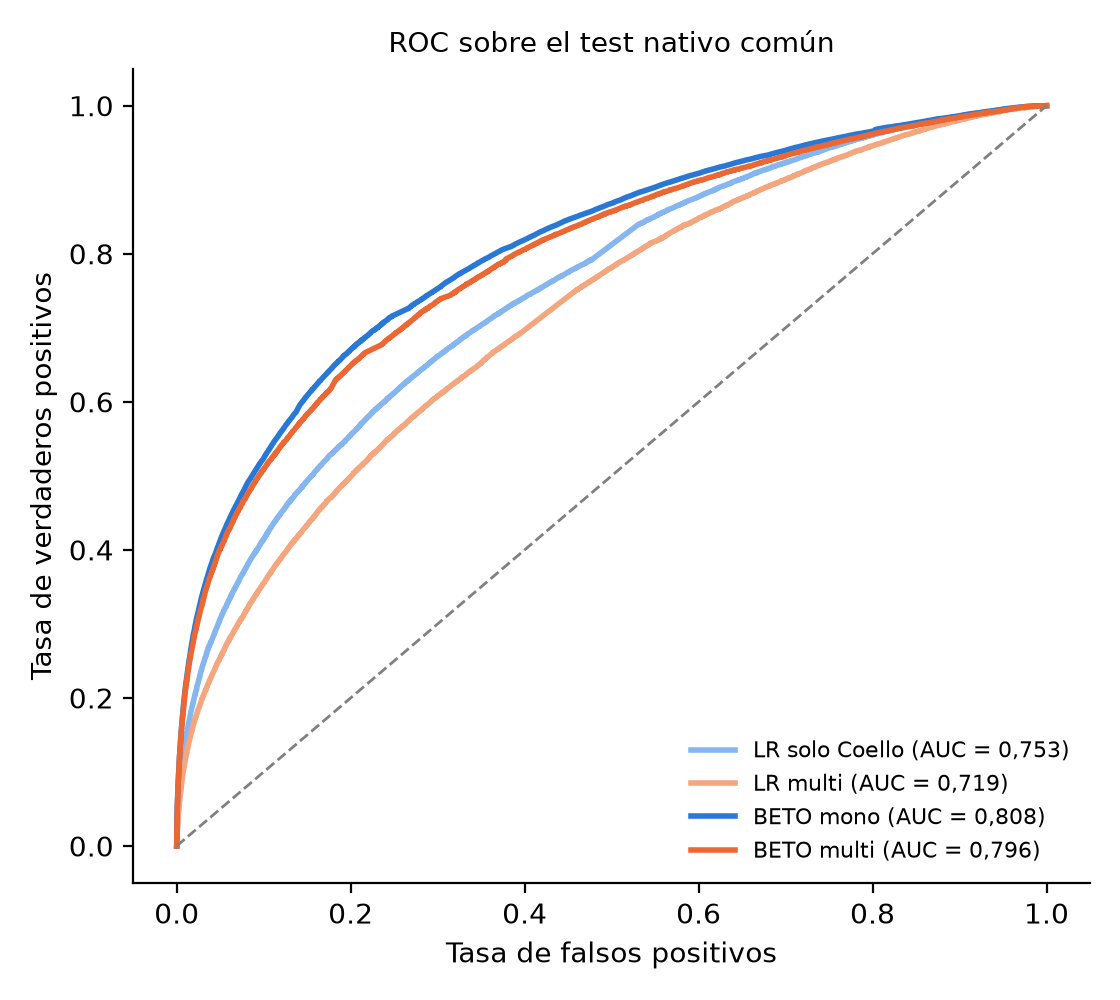
\includegraphics[width=\textwidth,height=0.48\textheight,keepaspectratio]{roc_test_nativo.png}
      \vskip-0.1cm
      {\tiny\color{ugrGris}Figura 2: Curvas ROC sobre el test nativo (BETO domina con AUC = 0{,}808).\par}
    \end{center}

    \column{0.50\textwidth}
    \begin{center}
      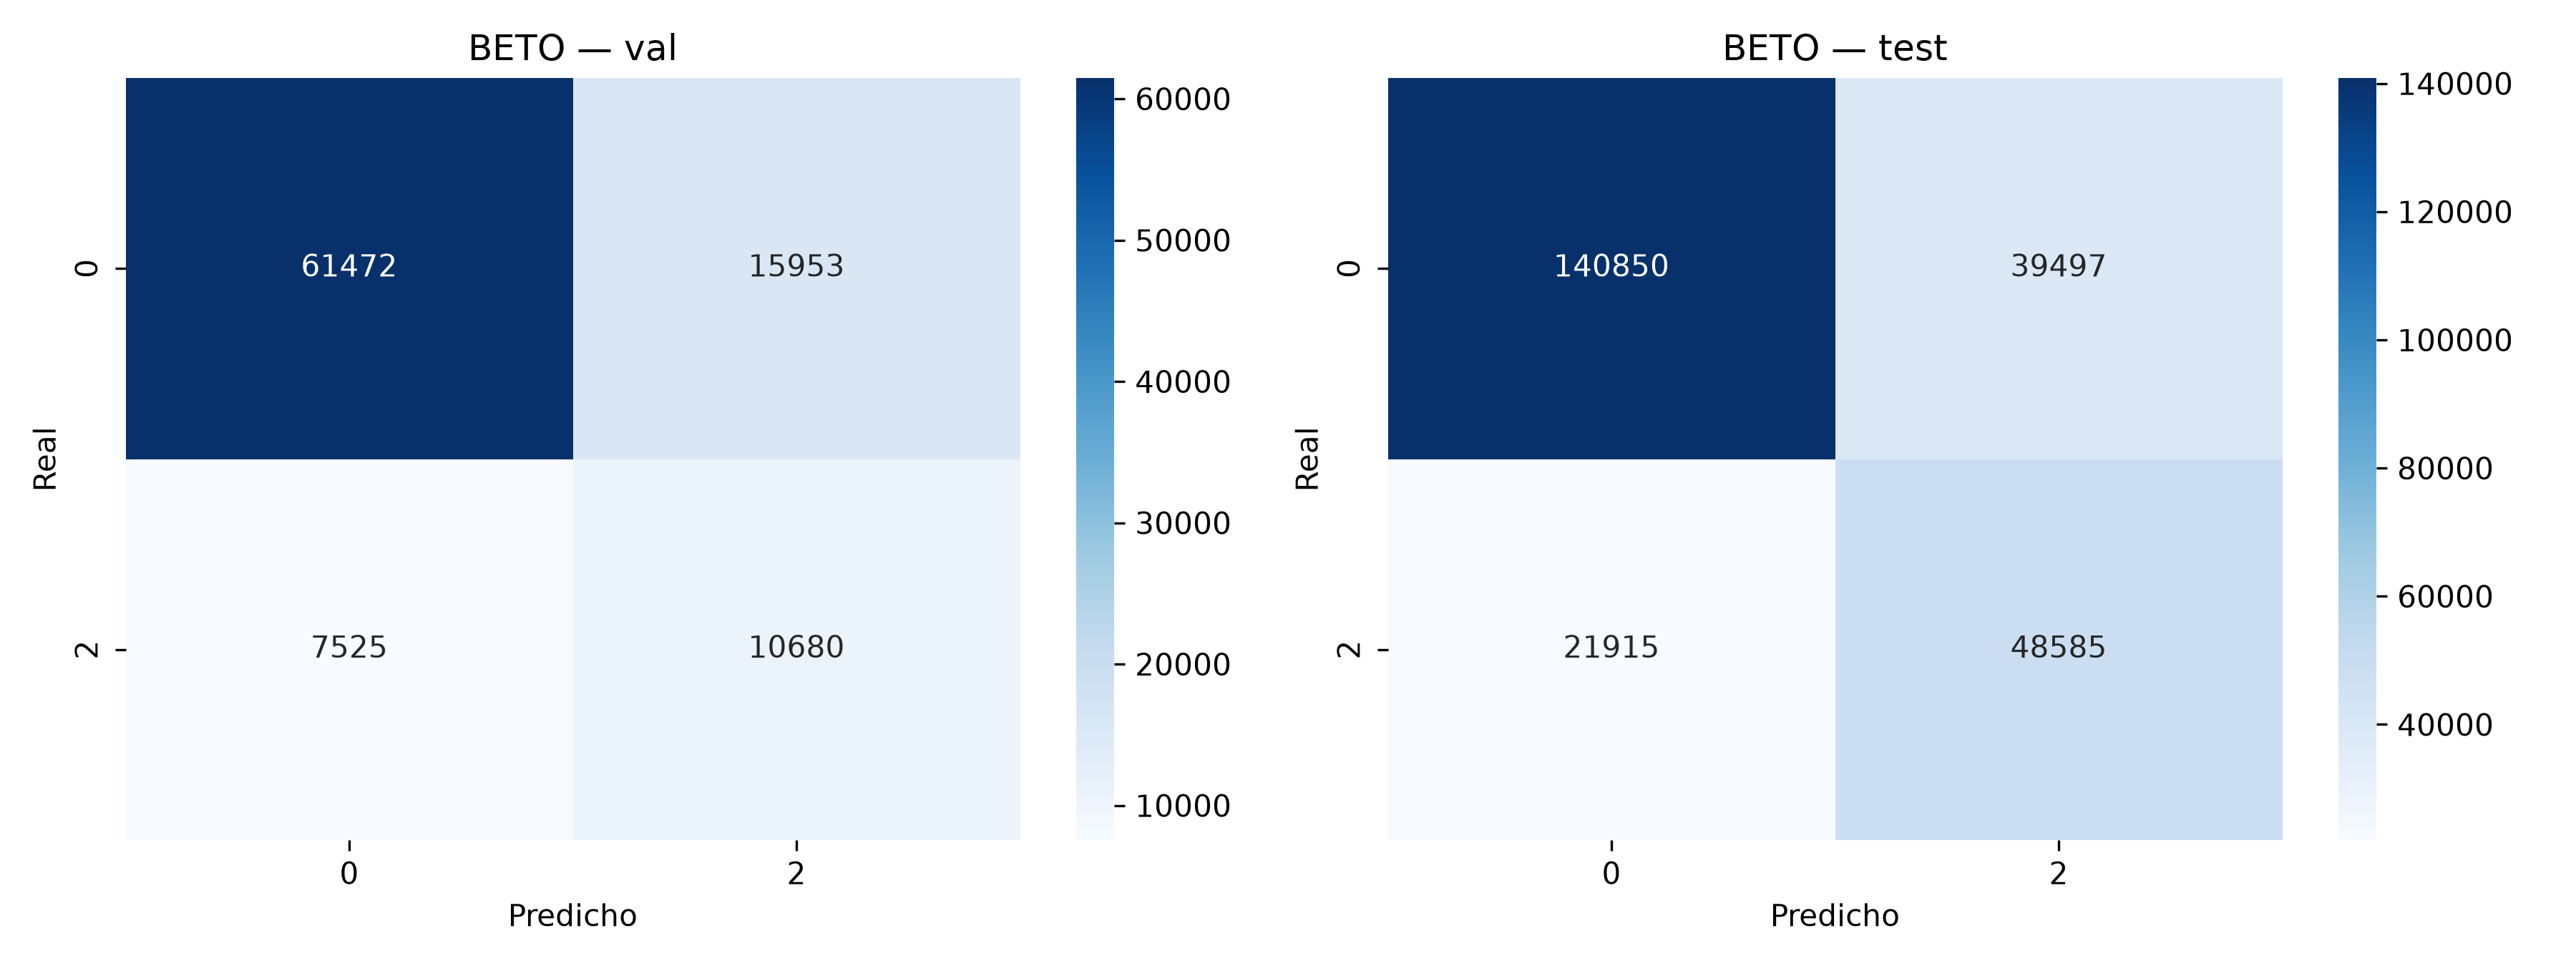
\includegraphics[width=\textwidth,height=0.48\textheight,keepaspectratio]{beto_confusion_matrix.png}
      \vskip-0.1cm
      {\tiny\color{ugrGris}Figura 3: Matriz de confusión normalizada de BETO mono (sensibilidad 69\,\%, especificidad 78\,\%).\par}
    \end{center}
  \end{columns}

  \vskip-0.1cm
  \begin{center}
    {\scriptsize\color{ugrAzul}\textbf{Compromiso clínico:} A nivel de publicación individual, la especificidad del 78\,\% minimiza falsas alarmas, mientras la agregación por perfil compensa falsos negativos.\par}
  \end{center}

  \note{
    La curva ROC de BETO domina de punta a punta a todas las líneas base. En la matriz de confusión observamos un equilibrio sólido: 78% de especificidad y 69% de sensibilidad sobre publicaciones aisladas. En cribado poblacional, este balance es óptimo para evitar saturar el sistema con falsos positivos.
  }
\end{frame}

% ---------------------------------------------------------------------
% Diapositiva 15: Contrastación Formal de Hipótesis
% ---------------------------------------------------------------------
\begin{frame}{Contrastación formal de la hipótesis ($H_1$ vs.\ $H_0$)}
  \framesubtitle{Diferencias pareadas directas e inferencia estadística conclusiva}

  \begin{table}
    \centering\scriptsize
    \setlength{\tabcolsep}{4pt}
    \caption{Diferencias pareadas ($\text{BETO} - \text{Línea Base}$) sobre las $2\,000$ réplicas de bootstrap.}
    \begin{tabular}{lcccc}
      \toprule
      \textbf{Comparación pareada} & $\boldsymbol{\Delta F_1}$\textbf{-macro} & $\boldsymbol{\Delta}$\textbf{AUC-ROC} & $\boldsymbol{\Delta\kappa}$ & $\boldsymbol{p}$\textbf{-valor empírico} \\
      \midrule
      BETO mono $-$ LR mono & \textbf{+0{,}062} \tiny{[0{,}038; 0{,}081]} & \textbf{+0{,}052} \tiny{[0{,}024; 0{,}077]} & \textbf{+0{,}116} \tiny{[0{,}068; 0{,}155]} & $p < 0{,}0005$ \\
      BETO mono $-$ SVM mono & \textbf{+0{,}063} \tiny{[0{,}040; 0{,}081]} & \textbf{+0{,}054} \tiny{[0{,}026; 0{,}077]} & \textbf{+0{,}119} \tiny{[0{,}072; 0{,}156]} & $p < 0{,}0005$ \\
      \bottomrule
    \end{tabular}
  \end{table}

  \vskip-0.1cm
  \ugrblockok{Decisión formal}{
    \begin{itemize}
      \item En el \textbf{100\,\% de las $2\,000$ réplicas} de remuestreo pareado por conglomerados de usuarios, BETO superó tanto a la Regresión Logística como a la SVM lineal.
      \item Los extremos inferiores del IC 95\,\% excluyen holgadamente el valor nulo ($\Delta F_1 > +0{,}038 > 0$).
      \item \textbf{Veredicto formal:} \textbf{Se rechaza $H_0$ y se acepta $H_1$} a nivel de publicación: BETO aporta una mejora predictiva estadísticamente demostrada y consistente.
    \end{itemize}
  }

  \note{
    La contrastación formal es contundente: réplica por réplica en el bootstrap pareado, BETO supera a las líneas base léxicas en el 100% de los casos. El extremo inferior del IC 95% para Delta F1-macro es de +0.038 y para Delta AUC de +0.024. Ambos son estrictamente mayores que cero. Se rechaza categóricamente H0 y se acepta H1.
  }
\end{frame}


% 6. Transferencia Translingüística y Nivel Usuario
% =====================================================================
% SECCIÓN 6: TRANSFERENCIA TRANSLINGÜÍSTICA Y NIVEL USUARIO
% =====================================================================

% ---------------------------------------------------------------------
% Diapositiva 17: Transferencia Translingüística
% ---------------------------------------------------------------------
\section{Transferencia y nivel usuario}

\begin{frame}{Efecto de la transferencia translingüística (mono vs.\ multi)}
  \framesubtitle{Impacto de incorporar publicaciones traducidas del inglés}

  \begin{table}
    \centering\scriptsize
    \setlength{\tabcolsep}{5pt}
    \caption{Rendimiento desagregado por dominio de prueba (Nativo Twitter vs.\ Traducido Reddit).}
    \begin{tabular}{lcccc}
      \toprule
      & \multicolumn{2}{c}{\textbf{Test Nativo (Twitter, 250k textos)}} & \multicolumn{2}{c}{\textbf{Test Traducido (Reddit, 46k textos)}} \\
      \cmidrule(lr){2-3} \cmidrule(lr){4-5}
      \textbf{Modelo evaluado} & \textbf{F1-macro} & \textbf{AUC-ROC} & \textbf{F1-macro} & \textbf{AUC-ROC} \\
      \midrule
      LR mono (solo nativo) & 0{,}653 & 0{,}753 & 0{,}418 & 0{,}802 \\
      LR multi (nativo + traducido) & 0{,}648 & 0{,}719 & 0{,}834 & 0{,}962 \\
      \midrule
      BETO mono (solo nativo) & \textbf{0{,}717} & \textbf{0{,}808} & 0{,}415 & 0{,}801 \\
      BETO multi (nativo + traducido) & 0{,}701 & 0{,}796 & \textbf{0{,}934} & \textbf{0{,}986} \\
      \bottomrule
    \end{tabular}
  \end{table}

  \vskip-0.15cm
  \begin{columns}[T]
    \column{0.49\textwidth}
    \ugralert{Transferencia negativa hacia el nativo}{
      Agregar Reddit traducido \textbf{degrada levemente} el rendimiento en tweets nativos (BETO: 0{,}717 $\to$ 0{,}701). La traducción introduce sesgos de registro y longitud.
    }
    \column{0.49\textwidth}
    \ugrblockok{Imprescindible en el dominio traducido}{
      Para clasificar textos de Reddit, los datos traducidos son esenciales: BETO mono colapsa ($F_1 = 0{,}415$), mientras BETO multi alcanza $F_1 = 0{,}934$.
    }
  \end{columns}

  \note{
    Comparamos empíricamente el entrenamiento mono y multi: en el dominio nativo de Twitter, agregar datos traducidos no mejora y causa una ligera degradación de 1.6 puntos de F1. Sin embargo, para clasificar en el dominio traducido de Reddit, el entrenamiento multi es imprescindible: BETO mono cae a 0.415, mientras que BETO multi alcanza 0.934. Esto resalta el peligro metodológico de presentar una sola métrica agregada.
  }
\end{frame}

% ---------------------------------------------------------------------
% Diapositiva 18: Agregación a Nivel de Usuario
% ---------------------------------------------------------------------
\begin{frame}{Agregación a nivel de usuario: del texto al perfil}
  \framesubtitle{Evaluación agregada: promedio de probabilidades por autor (64 usuarios de prueba)}

  \begin{table}
    \centering\scriptsize
    \setlength{\tabcolsep}{6pt}
    \caption{Rendimiento predictivo agregando el puntaje medio por usuario en el test nativo.}
    \begin{tabular}{lcccc}
      \toprule
      \textbf{Modelo evaluado} & \textbf{F1-macro} & \textbf{Sensibilidad} & \textbf{Especificidad} & \textbf{AUC-ROC} \\
      \midrule
      LR mono (ponderado) & 0{,}925 & 0{,}895 & 0{,}956 & \textbf{0{,}991} \tiny{[0{,}972; 1{,}000]} \\
      SVM lineal mono & \textbf{0{,}943} & 0{,}895 & \textbf{0{,}978} & 0{,}989 \tiny{[0{,}967; 1{,}000]} \\
      BETO mono (contextual) & 0{,}888 & 0{,}842 & 0{,}933 & 0{,}982 \tiny{[0{,}954; 0{,}999]} \\
      \bottomrule
    \end{tabular}
  \end{table}

  \vskip-0.15cm
  \begin{columns}[T]
    \column{0.49\textwidth}
    \ugrblockok{Discriminación casi perfecta por perfil}{
      Al promediar cientos de textos por usuario (media de 3\,919 publicaciones), el AUC salta a \textbf{$\ge$ 0{,}98 en todos los modelos}.
    }
    \column{0.49\textwidth}
    \ugralert{La ventaja de BETO se diluye}{
      El agregado estadístico a gran escala actúa como un filtro que compensa el ruido individual; a nivel de perfil completo, las líneas base igualan a BETO.
    }
  \end{columns}

  \note{
    Al agregar las predicciones por usuario promediando sus tweets, el AUC se dispara a 0.98 o más en todos los modelos. Sin embargo, surge un hallazgo fundamental: la superioridad de BETO se diluye a nivel de perfil completo, ya que el promediado masivo sobre miles de textos filtra los errores individuales de las líneas base lineales. BETO es diferencial cuando los textos son escasos o aislados.
  }
\end{frame}


% 7. Discusión, Limitaciones, Trabajo Futuro y Conclusiones
% =====================================================================
% SECCIÓN 7: DISCUSIÓN, CONCLUSIONES Y TRABAJO FUTURO
% =====================================================================

% ---------------------------------------------------------------------
% Diapositiva 19: Discusión y Aportes
% ---------------------------------------------------------------------
\section{Conclusiones y trabajo futuro}

\begin{frame}{Discusión integral y aportes de la investigación}
  \framesubtitle{Síntesis de los cuatro hallazgos empíricos y metodológicos principales}

  \begin{columns}[T]
    \column{0.49\textwidth}
    \ugrblockok{1. Superioridad contextual demostrada}{
      BETO supera a los modelos léxicos a nivel de documento ($\Delta F_1 = +0{,}062$, $\Delta\text{AUC} = +0{,}052$, $p < 0{,}0005$). Los 19 rasgos manuales no superan a los n-gramas puros.
    }
    \vskip0.05cm
    \ugrblock{2. Límites de la traducción automática}{
      La traducción neuronal expande la cobertura hacia comunidades de foros ($F_1 = 0{,}934$), pero no transfiere mejoras al dominio nativo de microtexto ($0{,}701$ vs.\ $0{,}717$).
    }

    \column{0.49\textwidth}
    \ugrblock{3. Eficiencia en el balanceo}{
      El submuestreo balanceado 50/50 alcanza un desempeño equivalente a la ponderación de pérdida utilizando un 40\,\% menos de datos, optimizando recursos computacionales.
    }
    \vskip0.05cm
    \ugralert{4. La unidad de análisis importa}{
      En publicaciones individuales aisladas, BETO es ampliamente superior. En perfiles completos con miles de publicaciones, el agregado estadístico equipara el rendimiento (AUC $\ge 0{,}98$).
    }
  \end{columns}

  \note{
    Sintetizamos los cuatro aportes cardinales: demostración de la superioridad de BETO en textos breves; límites empíricos del aumento por traducción; eficiencia del balanceo de clases; y el impacto decisivo de la unidad de análisis entre publicaciones aisladas y perfiles acumulados por usuario.
  }
\end{frame}

% ---------------------------------------------------------------------
% Diapositiva 20: Limitaciones del Estudio
% ---------------------------------------------------------------------
\begin{frame}{Limitaciones de la investigación y consideraciones éticas}
  \framesubtitle{Transparencia metodológica sobre el alcance real del sistema}

  \begin{columns}[T]
    \column{0.49\textwidth}
    \ugralert{Limitaciones metodológicas y técnicas}{
      \begin{itemize}
        \item \textbf{Sin validación clínica individual:} Etiquetas derivadas de redes sociales, no de entrevistas diagnósticas estructuradas (SCID-5 / MINI).
        \item \textbf{Sesgo de autoselección:} Los usuarios activos en redes no representan a la población clínica general.
        \item \textbf{Restricciones de hardware:} GPU local de 8\,GB VRAM limitó el ajuste a 128 tokens y 3 épocas, posponiendo validación cruzada 5-fold en BETO.
      \end{itemize}
    }

    \column{0.49\textwidth}
    \ugrblock{Compromiso ético y privacidad}{
      \begin{itemize}
        \item \textbf{Herramienta no diagnóstica:} Concebida como apoyo al cribado poblacional y vigilancia analítica, nunca como sustituto del criterio médico profesional.
        \item \textbf{Privacidad por diseño:} Anonimización estricta e irreversible mediante hash criptográfico (SHA-256) sin reidentificación de sujetos.
        \item \textbf{Uso responsable:} Delimitación clara del alcance para prevenir decisiones autónomas automatizadas sobre individuos.
      \end{itemize}
    }
  \end{columns}

  \note{
    Asumimos con rigor las limitaciones del trabajo: las etiquetas de redes no equivalen a un diagnóstico clínico formal, y las restricciones de GPU acotaron los modelos probados. Subrayamos que un clasificador de aprendizaje automático solo puede operar como herramienta de apoyo preliminar y nunca debe sustituir el juicio clínico profesional.
  }
\end{frame}

% ---------------------------------------------------------------------
% Diapositiva 21: Trabajo Futuro
% ---------------------------------------------------------------------
\begin{frame}{Líneas de trabajo futuro}
  \framesubtitle{Oportunidades de continuidad y extensión de la investigación}

  \begin{columns}[T]
    \column{0.49\textwidth}
    \ugrblock{1. Modelado y validación clínica}{
      \begin{itemize}
        \item \textbf{Adaptación continua de dominio:} Preentrenamiento no supervisado sobre corpus de salud mental previos al fine-tuning.
        \item \textbf{Validación clínica certificada:} Evaluación sobre cohortes con instrumentos estandarizados (PHQ-9 o DAIC-WOZ).
      \end{itemize}
    }

    \column{0.49\textwidth}
    \ugrblock{2. Temporalidad y explicabilidad}{
      \begin{itemize}
        \item \textbf{Detección temprana secuencial:} Modelado longitudinal (protocolo eRisk) para medir latencia mínima de alertas.
        \item \textbf{Interpretabilidad profunda:} Métodos de atribución (SHAP, Integrated Gradients) y análisis de atención en BETO.
      \end{itemize}
    }
  \end{columns}

  \note{
    Planteamos cuatro líneas de continuidad prioritarias: esquemas de preentrenamiento continuo adaptativo; validación con cohortes clínicas certificadas; modelado secuencial temporal según el estándar de eRisk; y métodos avanzados de explicabilidad en modelos Transformer.
  }
\end{frame}

% ---------------------------------------------------------------------
% Diapositiva 22: Conclusiones Finales
% ---------------------------------------------------------------------
\begin{frame}{Conclusiones finales}
  \framesubtitle{Cierre de la defensa de tesina de grado}

  \ugrblockok{Respuesta a la pregunta central de investigación}{
    \textbf{Es viable y ventajoso} emplear modelos contextuales preentrenados en español (BETO) para detectar indicios de depresión en publicaciones individuales, superando en más de 6 puntos de $F_1$-macro a los métodos clásicos con significancia estadística comprobada ($p < 0{,}0005$).
  }

  \vskip0.1cm
  \begin{itemize}
    \item \textbf{Aporte al estado del arte en español:} Se consolidó un benchmark riguroso, reproducible y abierto con más de 1{,}3 millones de documentos evaluados bajo particiones limpias por usuario.
    \item \textbf{Aporte metodológico crítico:} Se demostró que la traducción automática expande dominios pero no transfiere mejoras al dominio nativo, y que la unidad de análisis es crítica: la ventaja contextual de BETO en textos breves individuales se equipara con modelos lineales al evaluar perfiles de usuario agregados (AUC $\ge 0{,}98$).
    \item \textbf{Replicabilidad garantizada:} Repositorio con código modular, pipelines de preprocesamiento, configuraciones y predicciones disponibles para su verificación.
  \end{itemize}

  \note{
    En conclusión: BETO demuestra una ventaja representacional indiscutible en publicaciones individuales. Sin embargo, la mayor contribución de esta tesina radica en su rigor metodológico: demostrar el impacto de la partición por usuario y cómo la unidad de análisis modifica las conclusiones entre publicaciones individuales y perfiles acumulados.
  }
\end{frame}

% ---------------------------------------------------------------------
% Diapositiva 23: Cierre y Agradecimientos
% ---------------------------------------------------------------------
\begin{frame}[plain]
  \begin{tikzpicture}[remember picture,overlay]
    \fill[ugrAzul] (current page.north west) rectangle (current page.south east);

    \node[anchor=center] at (current page.center) {
      \begin{minipage}{0.85\textwidth}
        \centering
        
\includegraphics[height=1.1cm]{logo_ugr.png}\par\medskip
        {\fontsize{22}{26}\selectfont\bfseries\color{white} ¡Muchas gracias por su atención!}\par\medskip
        {\fontsize{12}{15}\selectfont\color{ugrCeleste!40} Preguntas, comentarios y discusión}\par\medskip
        {\color{white}\rule{0.65\textwidth}{0.8pt}}\par\medskip
        {\footnotesize\color{white}
          \textbf{Giuliano Crenna} \quad · \quad \textbf{Bruno Emmanuel Pace}\\[3pt]
          Licenciatura en Ciencia de Datos · Universidad del Gran Rosario (2026)\\[6pt]
          \color{ugrCeleste!30}\texttt{https://github.com/giulicrenna/Deteccion-Temprana-Depresion}
        }
      \end{minipage}
    };
  \end{tikzpicture}

  \note{
    Agradecemos a los evaluadores Jorge Fernández Acuña, Briant Gauna y Alejandro Hernández, a los docentes de la carrera y a la Universidad del Gran Rosario por su constante orientación. Quedamos a total disposición del tribunal para responder a sus preguntas y comentarios. Muchas gracias.
  }
\end{frame}


\end{document}
